\documentclass{beamer}

%%%%%%%%%%%%%%%%%%%%%%%%%%%%%%%%%%%%%%%%%%%%%%%%%%%%%%%%%%%%%%%%%%%%%%%
% Definicion de paquetes
% \usepackage{minted}
\usepackage[utf8]{inputenc}
\usepackage[spanish]{babel}
\usepackage{hyperref}
\usepackage{xargs}
\usepackage[nodayofweek,level]{datetime}
\usepackage[colorinlistoftodos,prependcaption,textsize=tiny]{todonotes}
\presetkeys{todonotes}{inline}{}
\usepackage{pgfpages}

%%%%%%%%%%%%%%%%%%%%%%%%%%%%%%%%%%%%%%%%%%%%%%%%%%%%%%%%%%%%%%%%%%%%%%%
% Definición de comandos
\setlength{\marginparwidth}{2cm}
% \unsure{I'm not sure}
\newcommandx{\unsure}[2][1=]{\todo[linecolor=red,backgroundcolor=red!25,bordercolor=red,#1]{#2}}
% \change{This must be changed}
\newcommandx{\change}[2][1=]{\todo[linecolor=blue,backgroundcolor=blue!25,bordercolor=blue,#1]{#2}}
% \info{Just information}
\newcommandx{\info}[2][1=]{\todo[linecolor=green,backgroundcolor=green!25,bordercolor=green,#1]{#2}}
% \improvement{THIS must be improved}
\newcommandx{\improvement}[2][1=]{\todo[linecolor=orange,backgroundcolor=orange!25,bordercolor=orange,#1]{#2}}
\newcommandx{\thiswillnotshow}[2][1=]{\todo[disable,#1]{#2}}
\newcommand{\mydate}{\formatdate{9}{12}{2021}}

\graphicspath{ {images/} }
%%%%%%%%%%%%%%%%%%%%%%%%%%%%%%%%%%%%%%%%%%%%%%%%%%%%%%%%%%%%%%%%%%%%%%%
% Beamer
\usetheme{Madrid}
% \AtBeginEnvironment{minted}{\fontsize{12}{12}\selectfont}
% \setbeameroption{show notes on second screen=right}
% \setbeameroption{show notes}
%%%%%%%%%%%%%%%%%%%%%%%%%%%%%%%%%%%%%%%%%%%%%%%%%%%%%%%%%%%%%%%%%%%%%%%
% Título
\title[SGDI]{RabbitMQ}
\author[S. García \and M. Ruiz]{Sergio García Sánchez \and Miguel Emilio Ruiz Nieto}
\date{\mydate}
%%%%%%%%%%%%%%%%%%%%%%%%%%%%%%%%%%%%%%%%%%%%%%%%%%%%%%%%%%%%%%%%%%%%%%%
%% Empieza el documento
\begin{document}
  \begin{frame}
    \titlepage
  \end{frame}

  \begin{frame}{Contenidos}
    \tableofcontents[hideallsubsections]
  \end{frame}

  \section{Introducción}
  \begin{frame}{Introducción}
    \begin{itemize}
      \item Los servicios web no tienen la capacidad de gestionar\\
      las peticiones que le llegan en un mismo momento
      \item<2-> Ejemplos:
      \begin{itemize}
        \item Web de venta de entradas ante un evento importante
        \item Servicio de videojuego online con alta demanda de
        usuarios
      \end{itemize}
      \item<3-> Como consecuencia:
      \begin{itemize}
        \item Caída del servicio
        \item Pérdida económica
        \item Pérdida de reputación
      \end{itemize}
    \end{itemize}
  \end{frame}

  \begin{frame}{Introducción}
    \onslide<+->{\begin{block}{Por tanto}
      Es necesario procesar las peticiones ``poco a poco''
    \end{block}}
    \onslide<+->{\begin{block}{Y para ello}
      Hay que implementar \textbf{una cola de mensajes}
    \end{block}}
  \end{frame}

  \begin{frame}{Introducción. Cola de mensajes}
    % \improvement{Desarrollar esta idea}
    \begin{itemize}
      \item Comuniación asíncrona \textit{service-to-service}
      usado en arquitecturas serverless y microservicios
      \item Permite desacoplar procesos con mucha carga de trabajo\\
      o almacenar trabajo \textit{en batch}
    \end{itemize}
    % A message queue is a form of asynchronous service-to-service\\
    % communication used in serverless and microservices architectures.\\
    % Messages are stored on the queue until they are processed and deleted.\\
    % Each message is processed only once, by a single consumer.\\
    % Message queues can be used to decouple heavyweight processing,\\
    % to buffer or batch work, and to smooth spiky workloads
  \end{frame}

  \begin{frame}{Cola de mensajes}
    \begin{figure}
      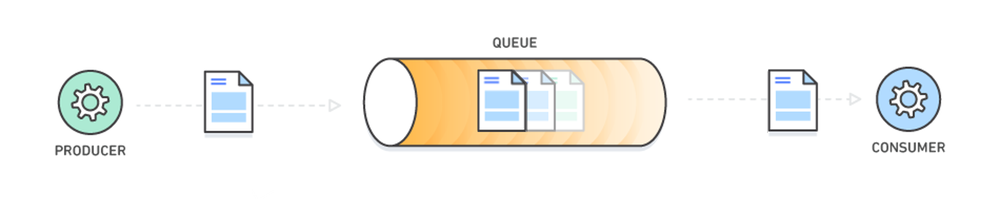
\includegraphics[width=\textwidth]{msg_queue.png}
    \end{figure}
  \end{frame}

  \begin{frame}{Ventajas}
    \begin{itemize}
      \item Mejor rendimiento
      \item Mayor fiabilidad
      \item Escalabilidad granular
      \item Desacoplamiento simplificado
    \end{itemize}
    \note{Desarrollar estos puntos}
  \end{frame}

  \begin{frame}{Colas de mensajes. Tipos}
    \begin{itemize}
      \item STOMP
      \begin{itemize}
        \item El protocolo más sencillo
        \item Implementado sobre HTTP
        \item Basado en intercambio de \textit{frames}
        \item La infraestructura de queues, topics y exchanges\\
        quedan del lado del cliente
      \end{itemize}
      \item MQTT
      \begin{itemize}
        \item Más ligero que STOMP
        \item Construído sobre TCP/IP
        \item Orientado a arquitecturas IoT
        \item Esquema \textit{publisher-suscriber} síncrono
      \end{itemize}
    \end{itemize}
  \end{frame}

  \begin{frame}{Colas de mensajes. Tipos}
    \begin{itemize}
      \item AMQP
      \begin{itemize}
        \item Comunicación asíncrona \textit{publisher-suscriber} mediante \textbf{broker}
        \item Permite el almacenamiento de mensajes
        \item Proporciona balanceo de carga
      \end{itemize}
    \end{itemize}
  \end{frame}

  \begin{frame}{Colas de mensajes. AMQP}
    \begin{figure}
      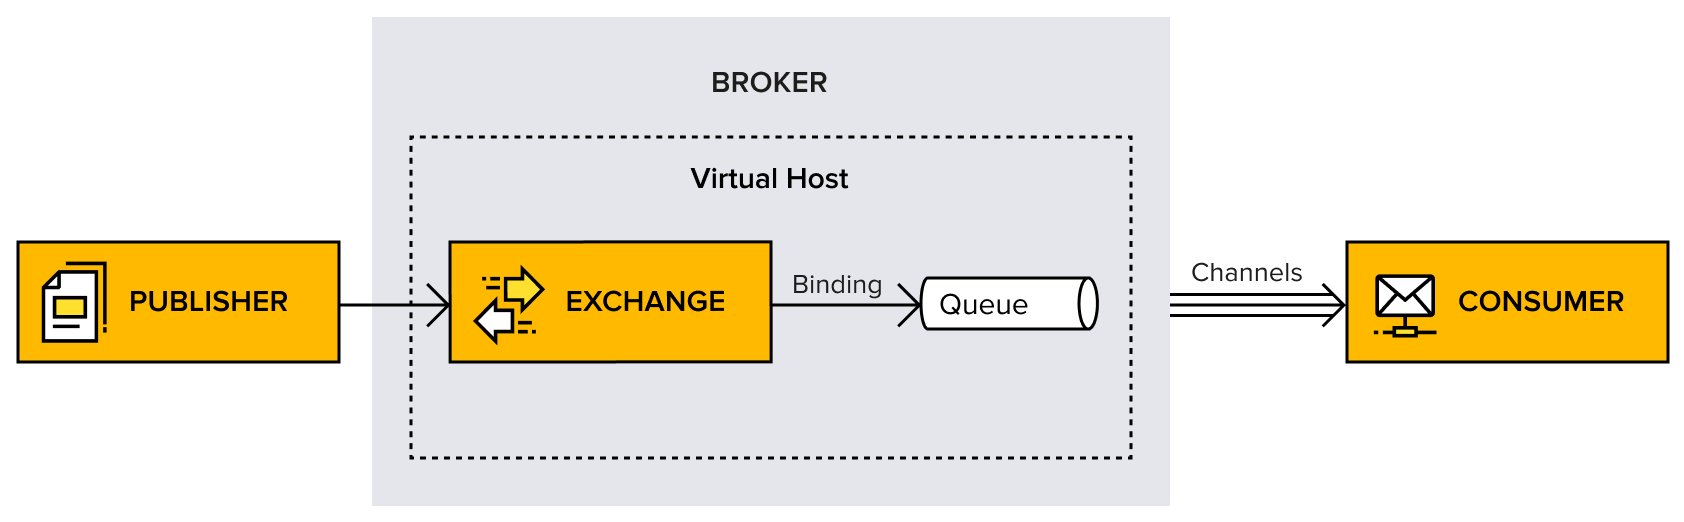
\includegraphics[width=\textwidth]{amq_concepts.png}
    \end{figure}
  \end{frame}

  \section{RabbitMQ}
  \begin{frame}{RabbitMQ. Introducción}
    \begin{itemize}
      \item Implementación del broker AMQP en Erlang
      \item Ofrece soporte para HTTP, STOMP y MQTT
      \item Interfaz web para manejar el broker y los componentes asociados
      \item Amplio soporte en múltiples lenguajes de programación
    \end{itemize}
  \end{frame}

  \begin{frame}{Exchanges}
    \begin{itemize}
      \item El primer componente que recibe el mensaje en AMQP
      \item Toma el mensaje y lo redirige a una o más colas
      \item Las colas se enlazan a los Exchanges mediante \textit{bindings}
      \item Se puede añadir un parámetro opcional \textbf{routing\_key}
    \end{itemize}
  \end{frame}

  \begin{frame}{Exchanges}
    \begin{block}{~\vspace{0.7cm}}
      \begin{center}
      \vspace{-0.65cm}
      \begin{tabular}{p{0.45\textwidth}|p{0.45\textwidth}}
        \textcolor{white}{\bf Tipo} & \textcolor{white}{\bf Descripción} \\
          Direct Exchange &  Envía el mensaje directamente a la cola basado en el routing\_key (amq.direct)\\ \hline
          Fanout Exchange &  Envía el mensaje a todas las colas enlazadas (amq.fanout) \\ \hline
          Topic Exchange &  Envía el mensaje a las colas suscritas al \textit{topic} (amq.topic)\\ \hline
          Headers Exchange & Envía el mensaje mirando las cabeceras en lugar del routing\_key (amq.headers)  \\
      \end{tabular}
      \end{center}
    \end{block}
  \end{frame}

  \begin{frame}{Topics}
    \begin{itemize}
      \item Se usan en los \underline{topic exchanges}
      \item Lista de palabras separadas por puntos
      \item Ejemplos:
      \begin{itemize}
        \item ``health.sports.football''
        \item ``\#.sports''
        \item ``sports.*''
      \end{itemize}
    \end{itemize}
  \end{frame}

  \begin{frame}{Dead Lettering}
    \begin{itemize}
      \item Ciertos mensajes pueden no ser consumidos por los consumers
      \item RabbitMQ ofrece mecanismos para gestionar el \textit{Dead lettering}
      \begin{itemize}
        \item Rechazo por TTL excedido
        \item Rechazo por exceso de longitud de mensaje
        \item Rechazo por parte del propio consumer (basic.reject)
      \end{itemize}
      \item Los mensajes son introducidos en un \textit{Dead letter exchange} (DLX)
    \end{itemize}
  \end{frame}

  \begin{frame}{RabbitMQ vs Apache Kafka}
    \begin{block}{~\vspace{0.7cm}}
      \begin{center}
      \vspace{-0.65cm}
      \begin{tabular}{p{0.45\textwidth}|p{0.45\textwidth}}
        \textcolor{white}{\bf RabbitMQ} & \textcolor{white}{\bf Apache Kafka} \\
        Broker de mensajería AMQP & Plataforma de procesamiento de flujo de eventos\\ \hline
        Utiliza protocolos de mensajería & Utiliza modelo editor/suscriptor \\ \hline
        Se pueden perder mensajes & No se pueden perder mensajes \\ \hline
        Enfocado a comunicación entre arquitecturas microservicios & Enfocado a Big Data
      \end{tabular}
      \end{center}
    \end{block}
  \end{frame}

  \section{Ejemplos prácticos}
  \begin{frame}{Ejemplos prácticos}
    \begin{itemize}
      \item AMQP - Uso de los exchanges y Dead Lettering
      \item STOMP over WebSocket
    \end{itemize}
  \end{frame}

  \section{Conclusiones}
  \begin{frame}{Conclusiones}
    \begin{itemize}
      \item Es necesario utilizar un mecanismo de cola de mensajes si
      la aplicación requiere de procesar un número grande de peticiones
      \item RabbitMQ ofrece soporte para diferentes lenguajes de programación
      dentro de su implementación
    \end{itemize}
  \end{frame}

  \section{Bibliografía}
  \begin{frame}{Bibliografía}
    \begin{itemize}
      % \item STOMP Protocol Specification \url{https://stomp.github.io}
      % \item MQTT Essentials - A Lightweight IoT Protocol
      \item RabbitMQ Documentation \url{https://www.rabbitmq.com/documentation.html}
      \item RabbitMQ Essentials
      \item Learn RabbitMQ: Asynchronous Messaging with Java and Spring
    \end{itemize}
  \end{frame}
\end{document}
